\documentclass{article}
\usepackage{graphicx} % Required for inserting images
\usepackage{graphicx} % Required for inserting images
\usepackage[left=0.5in, right=0.5in, top=0.5in, bottom=0.5in]{geometry}
\usepackage{amsmath}
\usepackage{amssymb}
\usepackage{amsfonts}
\usepackage{amsthm}
\usepackage{ulem}

\date{}

\begin{document}
\fontsize{14}{16} \selectfont

\text{Fractions, Decimals and Percentage.} \qquad Name: \hspace{5cm}  Class: \hspace{5cm}  \\
\vspace{20pt} 
\textit{(You must show your working.)  }
\vspace{5pt}

\hline
\vspace{10pt}
\text{(1) \quad What is} $ 47\% $ \text{written as a fraction?} 
\vspace{100pt}

\hline
\vspace{10pt}
\text{(2)} \quad $ \frac{2}{3} + \frac{3}{5} $  
\vspace{110pt}

\begin{center}
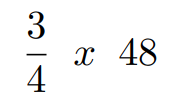
\includegraphics[width=5cm,height=3cm,label=fig:a]{a.png}
\end{center}

\section{My Image}

\begin{figure}[h] % 'h' for here, 't' for top, 'b' for bottom, etc.
  \centering
  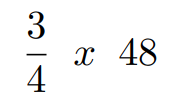
\includegraphics[width=5cm\textwidth]{a.png} % Adjust the width as needed
  \caption{My caption}
  \label{fig:my_label}
\end{figure}

\[
\frac{3}{\fbox{\hspace{1em}}} % 1em box width, adjust as needed
\]

\[
\frac{3}{\fbox{\makebox[1em]{\rule{0pt}{2em}}}} % 1em box width and 2em height, adjust as needed
\]

\[
\frac{3}{\fbox{\makebox[1em]{\rule{0pt}{1em}}}} % 1em box width and 2em height, adjust as needed
\]

\[
\genfrac{}{}{1pt}{0}{3}{\fbox{\makebox[1em]{\rule{0pt}{2em}}}} % 1pt line thickness
\]

\[
\genfrac{}{}{1.5pt}{0}{2}{\fbox{\makebox[1em]{\rule{0pt}{1em}}}} % 3pt line thickness
\]

\section{fbox below}
\[
\genfrac{}{}{1.5pt}{0}{2}{\fbox{\makebox[1em]{\rule{0pt}{1em}}}} % 3pt line thickness
\]

\section{fbox on top}
\[
\genfrac{}{}{1.5pt}{0}{\fbox{\makebox[1em]{\rule{0pt}{1em}}}}{2} % 3pt line thickness
\]



\end{document}